\chapter{Szabályzó kiválasztása és analízise}\label{chap:control}

A fejezetben a Simulinkben átviteli függvényre megtervezem a szabályzást. A szabályzó választásakor világossá vált, hogy egy egyszerű PID típusú szabályzás nem képes a rendszert jól kezelni. Igaz, hogy a PID közismert és az iparban egyszerűsége miatt széles körben használt, de épületgépészeti alkalmazásnál egy szabályzás jóságát többféleképp is értelmezhetjük\footnote{Mást tekintünk jó szabályzásnak egy tisztatérben, egy irodában, vagy egy nagyelőadóban, hiszen mások a felmerülő igények, és így a kritériumok is.}. Egyes esetekben hibahatárt megszabva lazíthatunk például a referenciakövetési feltételeken.

Az identifikált modellre többféle szabályzót tervezek, illetve próbálok ki.

A hasonló feladatokra leggyakrabban modell-prediktív (MPC) szabályzást használnak \cite{AFRAM2014343}. Ehhez szükség van a szakasz modelljére, ami alapján a szabályzó szimulálhatja a szakasz kimenetét. Az MPC egy beavatkozójel kiadása előtt több mintavételi perióduson, egy predikciós horizonton keresztül fut le, minden lehetséges  beavatkozójel-sorozatra a kimenetet szimulálva.
%A csúszóablak miatt receding horizon control
Ezen sorozatok közül a legjobbat kiválasztja és egy lépést végrehajt. Ezután a szimuláció újrakezdődik. A végrehajtott, adott horizonton optimális beavatkozójelet egy költségfüggvény minimalizálásával kapja. A költségfüggvényben különböző eltéréseknek vagy abszolútértékeknek különböző súlya lehet.

A szabályzás tehát képes egy horizontig előre tekinteni, és azon belüli optimális beavatkozást végrehajtani. (Az angol nyelvű irodalom erre \textit{receding horizon} névvel hivatkozik.) Az optimalizációt minden mintavételkor végrehajtja, így képes korrigálni, ha a jósolt kimenet és a tényleges kimenet eltérő.

A zárt szabályzási körben a stabilitás viszont nem garantált, erre külön módszerek léteznek (úgynevezett \textit{terminal cost}, azaz végső költség, illetve időben változó súlyozás). Mivel a vizsgált rendszerem nyílt körben is stabil, ezekkel nem kell foglalkoznom.

A stabilitás a beavatkozó jelek és a zavarjel (külső hőmérséklet) korlátosságából fakad. Ezeket is be lehet állítani a szabályzón, így az MPC a szelepekre csak 0 és 1 közötti beavatkozó jelet fog kiadni. A változások hatásait is figyelembe vehetjük, mivel a szelepeket 4-5 perc teljesen kinyitni.

A helyiség hőmérséklet-szabályozásakor a legfontosabb feladat a költségfüggvény súlyainak helyes beállítása\footnote{A súlyozást kiegészíthetik a fizikai korlátok is. Ha a szelepek nyitási- és zárási sebessége korlátos, akkor ezt nem lehet túllépni alacsony súly használatával sem.}. Ezek ugyanis befolyásolják a referenciakövetést - az állandósult állapotbeli hibát és lengést - és a beavatkozójel nagyságát, frekvenciáját is.

Az épületgépészeti rendszereknél a nagyobb frekvenciájú beavatkozójel könnyedén jelenthet alacsonyabb hatásfokot. Viszont ha megengedünk valamennyi ingadozást állandósult állapot körül, a terhelést kiegyenlíthetjük.
Egy irodában, vagy lakásban  például 0.1\si{\celsius}-os vagy 1\si{\celsius}-os pontosságú hőmérséklet-szabályzás közötti különbség komfortban aligha érezhető.
\vspace{6pt}

\begin{figure}[h]
	\centering
	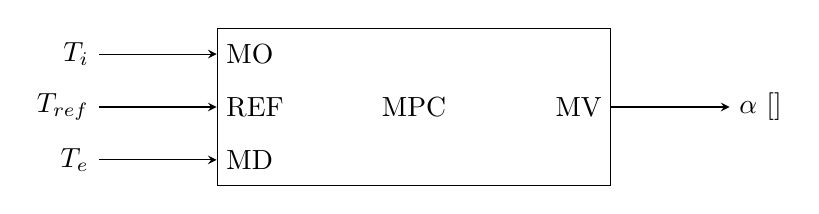
\begin{tikzpicture}[>=stealth]
	% Controller
	% ----------
	\node[draw,rectangle, minimum height=2cm,minimum width=5cm,
		  %label={[xshift=1.0cm, yshift=0.3cm]Label},
		  %label={[xshift=-4.1cm, yshift=-0.7cm]Label},
		  ]
		  (MPC) at (2.3,2.5) {\parbox{2cm}{\centering MPC}};	
	
	% az MPC doboz bemenetei
	\draw [<-] (MPC.165) node[right]{MO} -- +(-15mm,0) node[left]{$T_i$};
	\draw [<-] (MPC.180) node[right]{REF} -- +(-15mm,0) node[left]{$T_{ref}$};
	\draw [->] (MPC.0) node[left]{MV} -- +(15mm,0) node[right]{$\alpha$ [\si{\percent}]};
	\draw [<-] (MPC.195) node[right]{MD} -- +(-15mm,0) node[left]{$T_e$};
	
	\end{tikzpicture}

	\caption{Az MPC be- és kimenetei}
	\label{fig_mpcinout}
\end{figure}

\vspace{6pt}

\begin{table}[H]
	\footnotesize
	\centering
	%\renewcommand{\arraystretch}{2} % to increase cell height
	%\taburulecolor{gray}
	%\begin{tabular}{|p{0.8cm}|p{1cm}|p{1cm}|p{1cm}|p{1cm}|p{1cm}|p{1cm}|p{1cm}|}
	%
	%\begin{tabulary}{\linewidth}{LLc}
	\begin{tabu}{@{}cll@{}}
		\hline
		MPC 	& model predictive control 		& modell-prediktív szabályozás
		\\
		MO / OV	& measured output, output variable 	& mért kimenet (szabályzott jellemző)
		\\
		MD		& measured disturbance			& mért zavarás 
		\\
		MV		& manipulated variable			& beavatkozó jel
		\\
		REF 	& reference signal 				& referenciajel
		\\
		$T_s$ 	& sampling time					& mintavételi idő
		\\ 
		p 		& prediction horizon 			& predikciós horizont 
		\\ 
		c 		& control horizon				& szabályzási horizont
		\\
		J 		& cost function 				& költségfüggvény
		\\
		$w_u$ 	& weight (control signal) 		& beavatkozó jelet büntető együttható
		\\ 
		$w_{\Delta u}$ 	& weight (rate of control signal) 		& beavatkozó jel változását bünteti
		\\ 
		$w_y$ 	& weight (measured output) 		& hibajelet büntető együttható
		\\
		SF 		& scale factor 			& skálázási tényező
		\\    \hline
	\end{tabu}
	\label{tab:MPCvariables}
	\caption{A fejezetben ismertetett rövidítések és angol szakkifejezések}
	%
	%\label{tab:TabularExample}
	%\tabref{TabularExample}~táblázat
\end{table}
\vspace{10pt}



\section{Elvárások a szabályzás teljesítményével szemben}

Az MPC hangolása során % működését, tulajdonságait meg tudjam figyelni,
lépésről lépésre fogom módosítani az alapértelmezett paramétereket, azok hatását megfigyelem.
Az MPC szintézis folyamata a következő:% be kellene tabolni


\begin{enumerate}[noitemsep,topsep=0pt,parsep=2pt,partopsep=4pt,leftmargin=30pt]
	\item a szakaszt identifikálni kell, az átviteli függvény be- és kimeneteinek típusát be kell állítani,
	\item létre kell hozni az MPC-t a megfelelő mintavételi frekvenciával,
	\item be kell állítani a jelek fizikai korlátait és súlyukat a szabályzás költségfüggvényében,
	%\item Be kell állítani a jelek fizikai korlátait
	\item hozzá kell adni a Simulink modell saját változói közé (Model workspace) a szabályzót és megadni a nevét az Explicit MPC blokkjában (az itt található Review funciót is érdemes használni),
	\item be kell kötni a jeleket és le kell futtatni a szimulációt.
	
\end{enumerate}

%Identifikálni kell a szakaszt.

A \verb|"setmpcsignals()"| függvény használatával egy új átviteli függvényt hozunk létre, amit az MPC függvénynek odaadhatunk. Ez annyival több az identifikált átviteli függvénynél, hogy benne vannak a be-és kimenetek típusai is, aszerint, hogy az említett jelek milyen típusúak. A szakasz átviteli függvényének be-~és kimeneteit meg kell nevezni (\verb|MO, MD, MV|) Ezután az \verb|"mpc(tf, Ts)"| függvénnyel létrehozhatjuk az MPC szabályzót a megadott szakaszmodellre.



%Alapértelmezés szerint a költségfüggvény súlyai az alábbiak. A zárt szabályzási körben ezek a súlyok a hibajelet büntették a legjobban, ezért nagyon jó referenciakövetést sikerült elérni.
%
%
%Követelmények a referenciajelekre:
%
%Thermal comfort - Olesen, ISO EN 7730
%
%Floor temperature - herz-ől is
%


%Az MPC szabályzót létrehoztam a toolbox-szal, az identfikált szakaszból. Beállítottam a be-és kimenetek jellegét, korlátait. A ki-és bemeneteket helyesen bekötve már működött is a szabályzás.
%Fontos, hogy helyesen válasszuk meg a mintavételi időt, illetve a súlyokat

%A kezdeti cél egy "sima" szabályzás. Kérdés, hogy egyáltalán tud-e ilyet az MPC. Gyanítom, hogy a hibaminimalizáló függvény megfelelő megadásával tud: ha egy négyzetes hibaminimalizáló van rajta, \textit{biztosan "jó"} lesz.\footnote{Bármit is jelentsen a \textit{jó} szabályzás.}


%A fenti a klasszikus MPC, tov. info. Baochang DING, Modern MPC című könyvében olvasható.

\section{A létrehozott MPC tulajdonságai}

Az \verb|"mpc()"| függvény még nem ad azonnal használható szabályzót. Az alapértelmezett súlyok és a normalizálatlan bemenetek miatt a legkisebb költségű beavatkozás akár az is lehet, hogy a szabályzó nagy követési hiba ellenére nulla beavatkozó jelet ad ki.

A költségfüggvény akkor működik jól, ha a modellbemeneteket normáljuk. Be kell állítani az MPC mért változóinak tulajdonságánál a modell kimenetének  skálázását, amit az állandósult állapotbeli értékek, illetve a jellemző változásoknak megfelelően kell beállítani.

A helyiség modelljénél nagy eltérések vannak, hiszen a szelepek normálva vannak, a hőmérséklet értékeket viszont kelvinben értelmezem. Így a skálafaktort a 30..300 közötti nagyságrendben célszerű választani, mivel a hőmérsékletértékek nagyságrendileg \SI{30}{\degreeCelsius}-nyi tartományban változnak.

A Simulinkben identifikált modell egy munkapont körül (adott környezeti hőmérséklet mellett) volt csak pontos, ám ez a referenciakövetést nem rontotta el. A szabályzás megváltozott paraméterekkel is működött a Simscape hálózatra, a referenciakövetés minősége megmaradt.


%\begin{itemize}[noitemsep,topsep=-8pt,parsep=0pt,partopsep=0pt]
%	\item A mintavételi idő növelése az MPC-ben magával vonja, hogy az a Simulink blokkban is módosul. 
%	\item A Simulinkben az időt a jobb alsó sarokban mindig mp-ben írja ki. Ámde ha a steppingnél 1000 step-et állítok be, az a jobb alsó sarokban $T_s$-sel felskálázva fogja a mp-t mutatni. Azaz 5 perces sampling time esetén 1 step a jobb alsó sarokban T=300 mp-nek felel meg.
%	\item A mintavételi idő megválasztása nagyban meghatározza a költségfüggvény értékét.
%\end{itemize}



\subsection{Módosítások az MPC-ben}

A súlyozást módosítva adhatunk költséget a beavatkozásnak, csökkentve így pl. annak a frekvenciáját. Ez a referenciakövetést rontja, de esetünkben nem cél a tized \si{\celsius}-os pontosság, hanem az energiamegtakarítás.
Pontosan fel kellene ezért írni a forintosított költségét a beavatkozásnak, és ezt minimalizálni\footnote{\textit{Feng \cite{FENG2015199}} is szelepet használt, de az ott felírt költségfüggvényt nem pontosan értem.}. Ez viszont egy összetett kapcsolat és jelentősen függ az épületgépészettől. Így általánosan fogom a paraméterváltozások hatásait vizsgálni.

\subsection{Az MPC költségfüggvénye}


A szabályzó a predikciós horizonton belül minden lehetséges beavatkozójel-sorozatra kiszámolja annak (várható, modell szerinti) költségét. Azt a beavatkozójel-sorozatot választja, ami a legkisebb költséggel jár. Eztán a szabályzási horizontnak megfelelő számú beavatkozást végez, nem adja ki a teljes sorozatot. 

%A legbutább szabályzó szabályzási és predikciós horizontja is 1. Azaz egy lépéssel lát előre és a legkedvezőbb esethez (J költség minimális) tartozó beavatkozó jelet végrehajtja\footnote{Ezt formalizálni kellene egyenletben is.}. $J=w_u u + w_e e$, ahol a hibát a szabályzóban lévő szakaszmodell alapján számítjuk.
\textit{Agachi \cite{romanMPC_Agachi}} szerint:

\begin{equation} \label{eq_mpc_cost}
J = \sum_{i}^{p} \left(w_u \Delta u^2 + w_e (r_i-y_i)^2  \right)
\end{equation}

%(itt még csak $r_i=r$ állandó referenciajellel tudtam csinálni. )
ahol N a predikciós horizont, $w_u$ a beavatkozó jel változásának súlya, $w_e$ a hibajel súlya. A referenciajel jövőbeli változásait figyelembe lehet venni a predikciós horizonton belül\footnote{A jövőbeli változásokat ismerhetjük, ha van egy referenciajelünk, vagy lehet becslés rá egy időjárás-előrejelzés.\\Bővebben az elméletről: https://www.mathworks.com/help/mpc/ug/signal-previewing.html,\\illetve a felhasznált Simulink blokkok: https://www.mathworks.com/help/mpc/examples/improving-control-performance-with-look-ahead-previewing.html}.

A költségfüggvényben a hibajelhez és beavatkozó jelekhez, ill. azok változásaihoz különböző súlyok tartozhatnak.
Nagyobb súlyok nagyobb költséget eredményeznek, így a szabályzó a nagyobb költségű beavatkozójel-sorozatot kisebb valószínűséggel választja.

\begin{figure}[H]
		\centering
		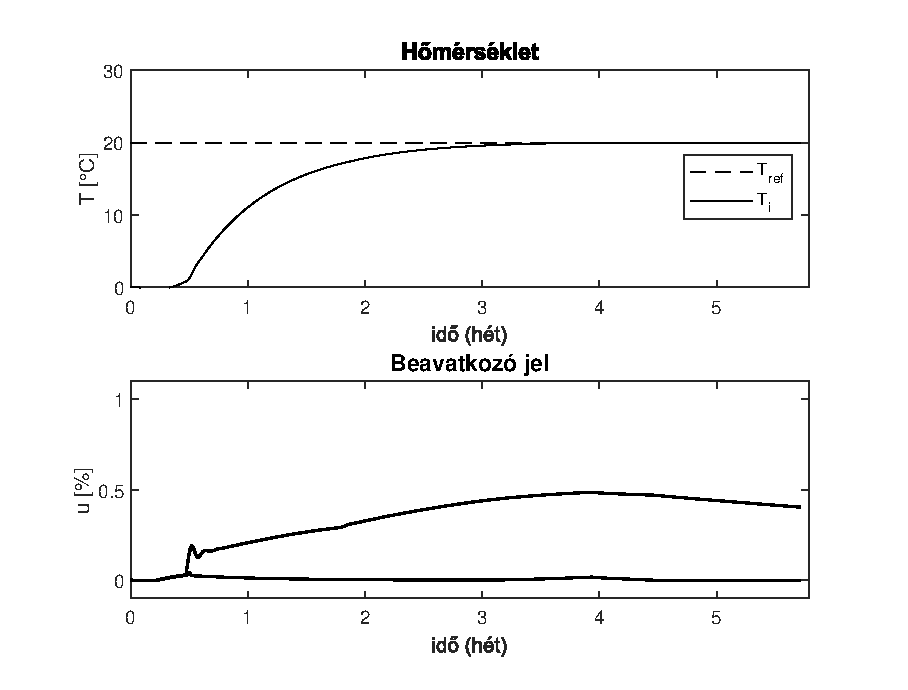
\includegraphics[width=0.8\textwidth]{figures/simscape/mpc}
		\caption{A zárt szabályzási kör ugrásválasza}
		\label{fig:mpc-simulated}
\end{figure}

A fenti ábrán látható a helyesen súlyozott MPC-vel a zárt szabályzási kör viselkedése. Ebben vannak tökéletlenségek, ezekre a fizikai modellnél térek majd rá. A szabályzóparaméterek az alábbi táblázatban láthatók.
\begin{table}[H]
	\footnotesize
	\centering
	%\renewcommand{\arraystretch}{2} % to increase cell height
	%\taburulecolor{gray}
	%\begin{tabular}{|p{0.8cm}|p{1cm}|p{1cm}|p{1cm}|p{1cm}|p{1cm}|p{1cm}|p{1cm}|}
	%
	%\begin{tabulary}{\linewidth}{LLc}
	\begin{tabu}{@{}cl@{}}
		\hline
		$T_s$ 	& 1800 s
		\\ 
		p 		& 50 minta (25 óra)
		\\ 
		c 		& 1
		\\
		$w_u$ 	& 0.005 
		\\ 
		$w_{\Delta u}$ 	& 50
		\\ 
		$w_y$ 	& 20
		\\
		SF 		& 30 
		\\   \hline
	\end{tabu}
	\label{tab:MPCfactors}
	\caption{MPC szabályzó paraméterei}
	%
	%\label{tab:TabularExample}
	%\tabref{TabularExample}~táblázat
\end{table}

\subsection{Fejlesztési lehetőségek a szabályzással kapcsolatban}
	
Épületautomatikai rendszerek használatával, például a fűtésszabályzás iContrALL intelligens otthon rendszerével a fellépő zavarásokat (emberek jelenléte, napsütés, szél) mérhetjük. A szabályzás a zavarások hatásmechanizmusának ismeretében jobb zavarelnyomást tud elérni, sőt az integrációval további beavatkozók is használhatók (például árnyékolástechnikai eszközök).

